\documentclass[10pt]{article}

% ARCHIVAL PAPER -- target venue J. Chem. Inf. Model. (ACS). Self-contained single-column
% article (US Letter, Times 10pt) with no external style-file dependency, so it compiles
% anywhere; swap in the achemso (JCIM) class at submission. Build: tectonic paper/foldgate_journal.tex
% This is the post-audit revision: 3 contributions (break+frontier / decomposition-as-diagnostic /
% priced repair), leakage-free headlines, notation + certificate-ledger + provenance tables,
% RMSD-conditioned utility, screening moved to SI as a cost result. See docs/JCIM_OUTLINE.md,
% docs/REVISION_TRIAGE.md, docs/REVISION_NUMBERS.md.
\usepackage[letterpaper,left=1.4in,right=1.4in,top=1in,bottom=1in]{geometry}
\usepackage{mathptmx}
\usepackage[T1]{fontenc}
\usepackage[utf8]{inputenc}
\usepackage{amsmath,amssymb}
\usepackage{booktabs}
\usepackage{graphicx}
\usepackage{caption}
\usepackage[dvipsnames]{xcolor}
\usepackage[numbers,sort&compress]{natbib}
\usepackage{titlesec}
\usepackage[hidelinks]{hyperref}

\captionsetup{font=small,labelfont=bf}
\titlespacing*{\section}{0pt}{6pt}{2pt}
\titlespacing*{\subsection}{0pt}{4pt}{1pt}
\titleformat{\section}{\normalfont\large\bfseries}{\thesection}{0.5em}{}
\titleformat{\subsection}{\normalfont\normalsize\bfseries}{\thesubsection}{0.5em}{}
\setlength{\parindent}{0pt}
\setlength{\parskip}{5.0pt}
\newcommand{\Real}{\mathbb{R}}

\title{\vspace{-2.2em}\textbf{\large Know When to Fold: Risk-Controlled Abstention for\\
Protein--Ligand Co-Folding under Novelty Shift}}
\author{Rikhin Kavuru\\ \small Independent Researcher \\ \small \texttt{rikhin@virahacks.com}}
\date{}

\begin{document}
\maketitle
\vspace{-2.4em}

\begin{abstract}
\small
Protein--ligand co-folding models (AlphaFold3, Boltz, Chai) report confidence scores that correlate
with pose accuracy, but correlation is not a decision rule, and it is weakest on the novel pockets and
chemotypes drug discovery cares about. We build \texttt{foldgate}, a training-free layer that turns
frozen co-folding confidence into a risk-controlled accept/abstain gate, and audit where its guarantee
fails. Calibrating on familiar targets and deploying on novel ones drives realized selective error to
$0.55$ against a $0.20$ target (AF3; $0.48$ to $0.66$ across five models). A per-stratum feasibility
analysis shows this is not a tuning problem: of $50$ model-by-stratum cells, $35$ admit \emph{no}
threshold on the frozen score that reaches the target at any coverage, robust to an exact binomial lower
bound, so abstention is the only certified action there. An exact decomposition of the realized risk
explains why and yields a measurable drift diagnostic that selects the repair from a labeled probe.
Group-conditional recalibration restores per-stratum control, retaining $73\%$ of AF3 poses at certified
risk $\le 0.20$ under leakage-free target-grouped cross-validation where the native gate retains $20\%$,
at a price we measure: a median of $38$ in-stratum labels on the familiar strata, and, on the novel tail,
no repair by stratification alone. A public deployment-computable proxy for the stratifier tracks the
oracle on low and moderate novelty but loosens control on the novel tail, so for closed-training models
the repair is deployable one stratum out and the extreme tail remains uncertifiable. The layer runs on
released predictions on CPU and ships as certificate cards per model and novelty stratum.
\end{abstract}

\section{Introduction}
Co-folding models predict a protein--ligand complex and emit confidence scores (interface predicted
TM-score, ipTM; ranking score; predicted aligned error). A practitioner who wants to act on a predicted
pose needs a decision rule that carries an error guarantee. Conformal selective prediction supplies one:
accept a pose when its score clears a threshold, abstain otherwise, and certify that the error rate among
accepted poses stays below a target $\alpha$ with high probability~\citep{vovk2005,geifman2017}. The catch
is that this guarantee assumes exchangeability, that a new target is statistically interchangeable with the
calibration examples, and that breaks precisely where deployment matters, on ligands and pockets dissimilar
to the training set. In drug-discovery terms the model is most overconfident on the never-before-seen
molecules a program cares about, so the operational question is not average accuracy but whether a single
delivered pose can be trusted.

We make three contributions, all training-free with respect to the co-folding model and all computed from
released predictions on CPU.
\textbf{(1)} We give a finite-sample selective-risk gate over frozen co-folding confidence, show its
guarantee collapses under novelty shift, and map the collapse with a per-stratum \emph{feasibility
frontier} that decays to zero on novel strata; reliability drift attributes the collapse to concept shift
(Sec.~\ref{sec:break}--\ref{sec:frontier}).
\textbf{(2)} We prove an exact decomposition of the realized selective risk into a covariate-corrected
reference and an accept-region concept gap that no training-free reweighting can move, turning it into a
measurable diagnostic that selects, from a labeled probe, which repair a deployment region admits
(Sec.~\ref{sec:decomp}).
\textbf{(3)} We repair what is repairable with group-conditional calibration and a label-free
worst-subpopulation certificate, match the certifier to the loss, and \emph{price} the repair: the label
cost as a design curve, a deployment-computable proxy stratifier, and the honest bottom line that the
extreme novel tail is uncertifiable by stratification alone (Sec.~\ref{sec:repair}). A leakage-free utility
evaluation and a decision-curve analysis follow (Sec.~\ref{sec:utility}).

The closest prior work is CoDrug~\citep{codrug}, which conformalizes a \emph{scalar} molecular property
under covariate shift with the same weighted-conformal tool~\citep{tibshirani2019} our decomposition shows
concept shift defeats in this domain; we are not aware of a prior conformal treatment of co-folding pose
correctness, or of training-set similarity used as the shift variable for it. Confidence-tracks-accuracy
studies for co-folding virtual screening~\citep{shen2026vs} rank by ipTM but supply neither a coverage
guarantee nor an abstention rule, which is the gap this layer fills. A reweighting-invariant selective-risk
floor of the same abstract character was shown independently and concurrently for LLM
abstention~\citep{crcgupta} (arXiv preprint, June 2026); ours is its co-folding specialization, localized
per novelty stratum with a matching in-stratum achievability bracket. Conformal
selection~\citep{jin2023selection,bai2026score} (the latter an arXiv preprint) is complementary: it certifies
which \emph{compounds} to advance given a labeled calibration set, while this layer certifies the
\emph{pose} correctness a co-folding screen rests on, training-free.

\section{Data and definitions}\label{sec:data}
\textbf{Unit and loss.} The decision-relevant unit is a delivered top-1 pose per system with a native
confidence $s$. The loss is $L=\mathbf{1}[\text{symmetry-corrected ligand-RMSD}>2\,\text{\AA}]$ against the
released BiSyRMSD label, so a certified selective risk is a bound on the accepted-set error rate. We use $L$
throughout (Table~\ref{tab:notation}). RMSD is the shipped symmetry-corrected BiSyRMSD (receptor
superposition, ligand-in-place); recomputed geometry is used only where noted (Table~\ref{tab:provenance}).

\textbf{Novelty axes.} We stratify by training-set similarity along two structural axes: a ligand axis
(ECFP4 Morgan Tanimoto to the nearest training ligand) and a pocket axis (SuCOS shape $\times$ pocket
query-coverage), both released by Runs N' Poses. Each axis is binned into quartiles $S_0$ (familiar) to
$S_3$, with systems that have no training analog (missing similarity, $30$--$34\%$ of poses) forming a
fifth no-analog stratum $S_4$. The quartile edges are fixed a priori from the similarity marginal;
Table~S1 lists $n$ and the similarity range each bin spans, per model and axis. We treat structural
similarity, not deposition recency, as the operative shift variable, for a reason the data forces
(Sec.~\ref{sec:break}).

\textbf{Cohort.} We evaluate five models
(AF3~\citep{af3}, Boltz-1, Boltz-1x~\citep{boltz}, Chai-1~\citep{chai}, Protenix~\citep{protenix}) on Runs
N' Poses~\citep{rnp}. Figure~\ref{fig:consort} is the reduction chain: $13{,}535$ raw delivered poses
(six models) minus the $933$ Boltz-2 poses used only as an ungoverned affinity comparator
(Sec.~\ref{sec:utility}) give $12{,}602$ governed poses over $2{,}425$ systems; deduplicating to one pose
per (system, model) gives $11{,}254$ independent target-labels for the five governed models. Certificates
that must be per deployed model use the target-label unit, since several ligand instances of one system
fail together and pooling them as independent draws is anti-conservative. The cohort is chemically diverse
and not a single-family monoculture: $55\%$ drug-like ($300$--$500$\,Da) with a $24\%$ fragment tail,
$2{,}412$ distinct receptors, and no PDB header class above $21\%$.

\textbf{Deployment cost.} The native-score gate is CPU-only and consumes one released prediction per
target. An optional combined score (a calibration-only gradient-boosted map from cheap per-prediction
features to $P(\text{correct})$: confidence, interface ipTM, ensemble spread, cross-model agreement,
PoseBusters validity, ligand descriptors) improves the operating point but consumes the five-sample
ensemble and cross-model features, so it needs $N$ model inferences per target. We report the native-only
guarantee prominently and flag the combined score as the upgrade. The combined score's cross-model features
are moderately correlated with novelty ($|\rho|$ up to $0.35$), so it is a partly novelty-aware re-score;
this is legitimate and places the \emph{combined} score on the achievability side of the theorem below,
which governs the frozen \emph{native} score.

\begin{table}[t]
\centering\small
\caption{Notation.}
\label{tab:notation}
\begin{tabular}{ll@{\hskip 2em}ll}
\toprule
$L$ & loss $\mathbf{1}[\text{RMSD}>2$\,\AA$]$ & $\alpha,\delta$ & risk target, failure prob.\ ($0.20,0.10$) \\
$s,\tau$ & score, accept threshold ($s\ge\tau$) & $c$ & coverage (accepted fraction) \\
$\nu, S_\nu$ & novelty axis, stratum & $\eta_P,\eta_Q$ & source/target error conditional $P(L{=}1\mid X)$ \\
$R_{\mathrm{ref}}$ & covariate-corrected reference risk & $\bar\Delta_c$ & accept-region concept gap \\
$D(\nu)$ & reliability drift at stratum $\nu$ & $m^\star,\beta^\star$ & certified min.\ subpop.\ mass, CVaR level \\
$\rho^\star$ & DRO robustness radius & $n_g$ & in-stratum labels \\
\bottomrule
\end{tabular}
\end{table}

\begin{table}[t]
\centering\small
\caption{Label provenance. The primary selective-risk results use the shipped BiSyRMSD label; only the
label-free danger-floor / cross-model consensus analysis (SI) uses recomputed pose geometry, on the
single-chain subset that App.~\ref{app:integrity} shows is the only frame that is trustworthy.}
\label{tab:provenance}
\begin{tabular}{lll}
\toprule
Result & Label / geometry & $n$ \\
\midrule
Break, frontier, repair, utility (Secs.~\ref{sec:break}--\ref{sec:utility}) & shipped BiSyRMSD & $11{,}254$ target-labels \\
Cross-model danger floor / consensus (SI) & recomputed, single-chain receptors & $6{,}163$ instances \\
Interaction-fingerprint recovery (Sec.~\ref{sec:utility}) & recomputed contacts vs.\ crystal & $11{,}711$ poses \\
\bottomrule
\end{tabular}
\end{table}

\begin{figure}[t]
\centering
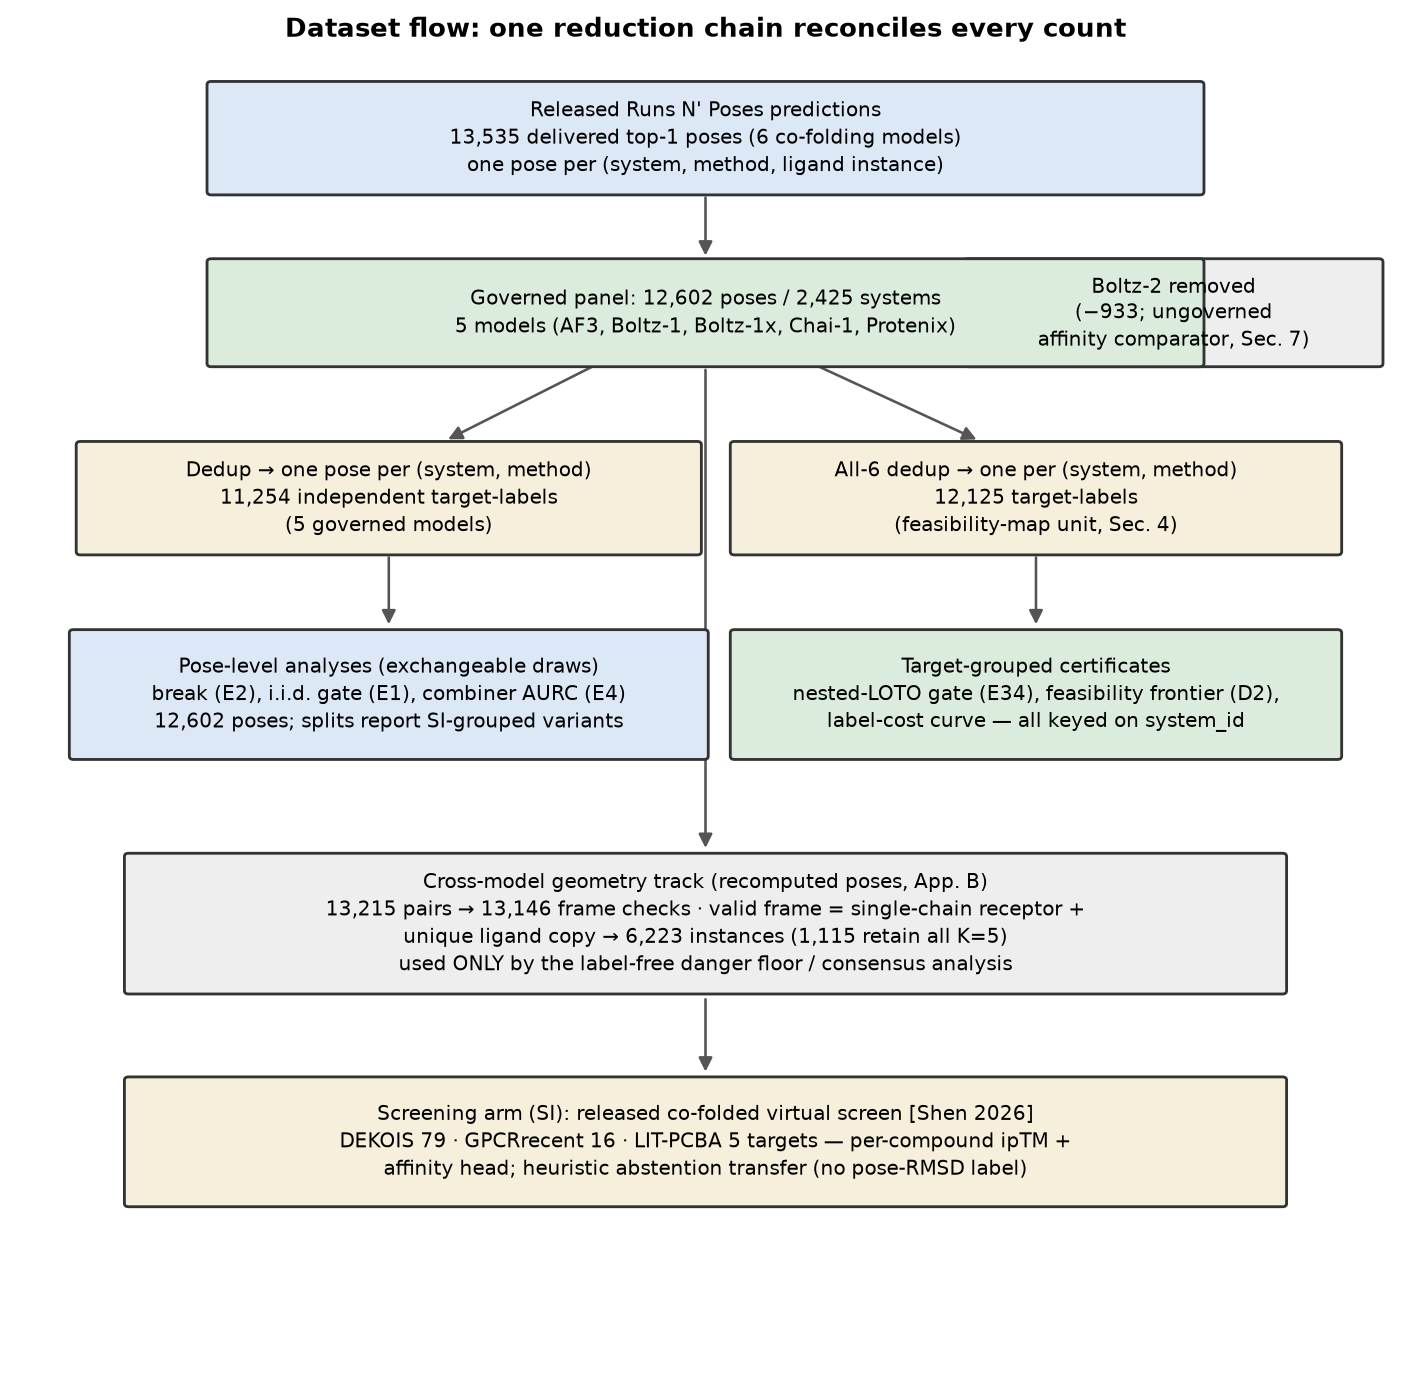
\includegraphics[width=0.82\textwidth]{../results/figures/consort_flow.png}
\caption{Dataset flow. One reduction chain reconciles every count; each node is annotated with the
experiments that consume it. Counts are recomputed live from the released predictions.}
\label{fig:consort}
\end{figure}

\textbf{Gate.} The gate accepts when $s\ge\tau$ and picks the largest accept set whose selective risk is
certified $\le\alpha$ by Learn-then-Test with fixed-sequence testing~\citep{angelopoulos2021ltt}, testing
each $H_0(\tau):P(L{=}1\mid s\ge\tau)\ge\alpha$ with an exact binomial tail along a pre-specified,
data-independent coverage grid (top-$k$ ranks, $c\in\{0.05,0.06,\dots,1.00\}$, fixed before any risk was
computed and archived in the repository). This gives $P(\text{selective risk}\le\alpha)\ge 1-\delta$,
finite-sample and distribution-free.

\section{The exchangeability break}\label{sec:break}
\textbf{The break.} A single global threshold hides severe per-stratum under-coverage. For AF3 the marginal
realized risk $R_{\mathrm{marg}}=0.177$ masks $R_{\mathrm{marg},S_3}=0.375$ on the novel ligand stratum
(Fig.~\ref{fig:break}, with Clopper-Pearson intervals and accepted $n$ per point). The operational failure
is starker: calibrating the gate on the familiar strata ($S_0,S_1$) and deploying on the novel tail
($S_3,S_4$) drives the realized error to $R_{\mathrm{transfer}}=0.55$ (AF3; $0.48$--$0.66$ across the five
models) against the $0.20$ target, so the certificate is inverted, not merely loose. We lead the break on
$S_3$; the no-analog $S_4$ (AF3 $n\!\approx\!76$, greyed in the figure) is small-sample and enters only in
the feasibility frontier, where zero coverage is the point.

\begin{figure}[t]
\centering
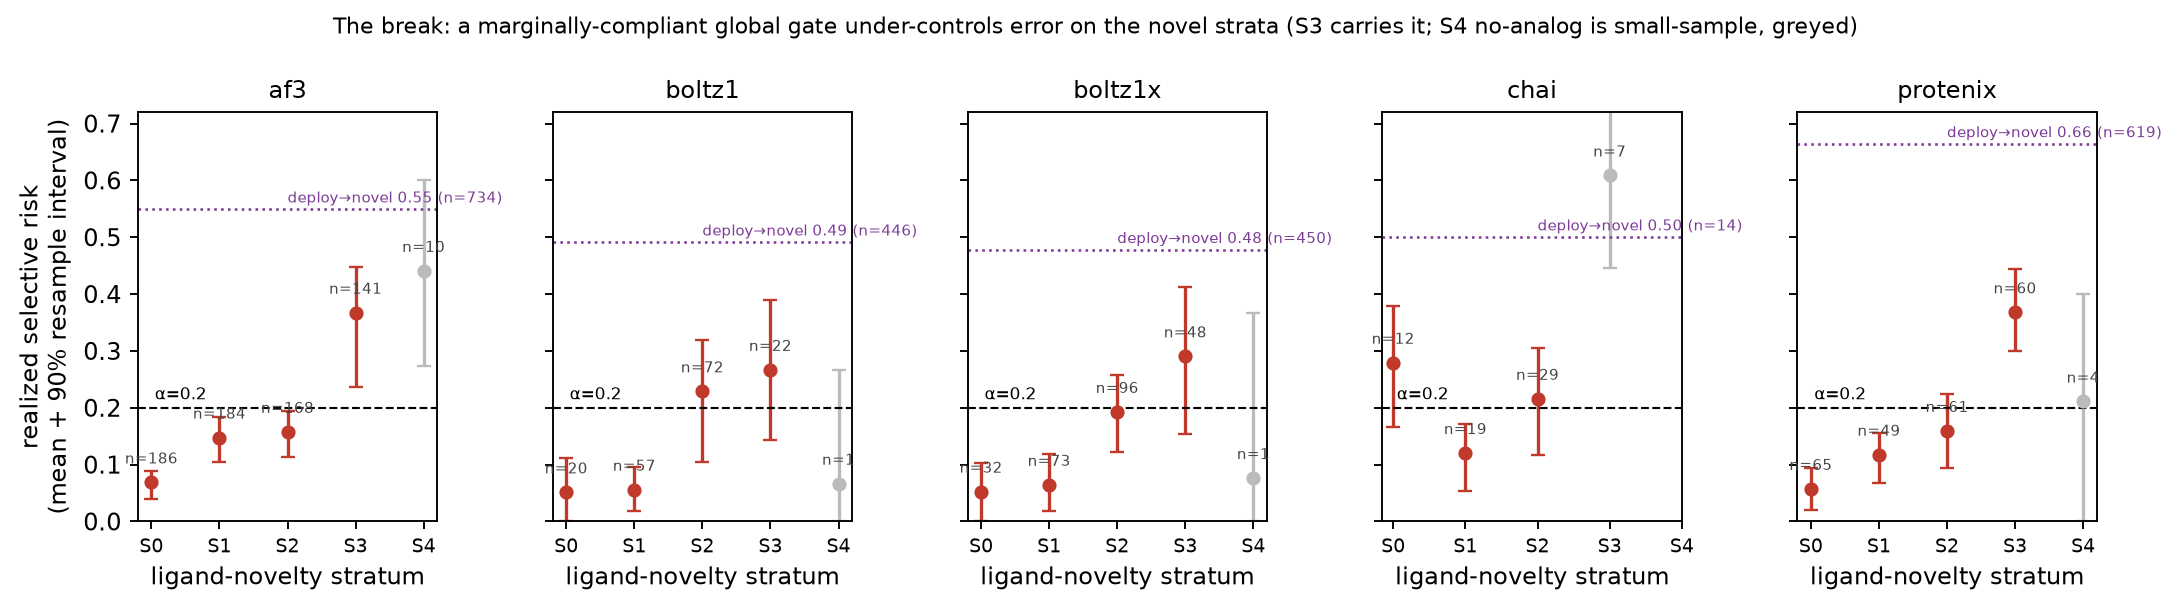
\includegraphics[width=0.98\textwidth]{../results/figures/break_money.png}
\caption{The break. Per-stratum realized selective risk of a marginally-compliant global gate, over $300$
target-grouped calibrate/deploy resamples (mean, $90\%$ resample interval, median accepted $n$ per point);
the no-analog $S_4$ is greyed as small-sample. Realized risk climbs above the target $\alpha=0.20$ as
ligand similarity falls, and the dotted line marks the calibrate-on-familiar / deploy-on-novel realized
risk (AF3 $0.55$). The break is carried by $S_3$.}
\label{fig:break}
\end{figure}

\textbf{Why it breaks: concept shift, not recency.} Weighted conformal would fix this if the shift were
pure covariate shift, where $P(L\mid s)$ is stable and only the marginal $P(s)$ moves. We test that by
measuring \emph{reliability drift}
$D(\nu)=\sum_{\text{bins}} w\,[\,P(L{=}0\mid s,S_0)-P(L{=}0\mid s,S_\nu)\,]$, the confidence-conditional
correctness gap between the familiar reference and stratum $\nu$. Drift is large on structural novelty and
its $90\%$ bootstrap interval excludes zero for every model (Protenix reaches $+0.63$ on pocket novelty,
Chai $+0.52$); the $+0.63$ is not a sparse-bin artifact, as every confidence quintile behind it holds
$\ge 103$ novel-pocket targets and the top-confidence bin still recovers to only $0.54$ correct against
$0.95$ on the familiar stratum. Confidence is optimistic on novel structure, the signature of concept
shift. A signed accept-region decomposition makes this quantitative: for AF3 on $S_3$ the target-risk gap
of $0.328$ splits into a concept term of $0.309$ ($90\%$ CI $[0.27,0.35]$) and a covariate term of $0.018$,
which Sec.~\ref{sec:decomp} turns into a theorem.

\textbf{The temporal axis is a benchmark artifact, not a null result.} Earlier framings contrasted a large
structural drift with a near-zero temporal drift. That contrast is real but must be stated precisely: every
Runs N' Poses structure is deposited after the $2021$-era models' training cutoff, so the temporal axis
ranks recency \emph{among already-out-of-training structures} rather than in- versus out-of-training, and a
flat drift there is a property of the benchmark, not evidence of temporal robustness. The one model with a
genuine within-benchmark cutoff boundary is Boltz-2 ($2023$-06-30); across it the reliability drift is
$+0.005$ ($90\%$ CI $[-0.075,0.079]$), and its structural $S_3$ break is unchanged whether keyed on the
$2021$- or the correctly-referenced $2023$-training similarity ($0.364$ vs.\ $0.367$ correct). Structural
similarity is therefore the operative shift variable, and we do not claim a temporal-generalization result.

\section{The feasibility frontier}\label{sec:frontier}
The break is a fixed-coverage statement; it leaves open whether $\alpha$ is reachable by lowering coverage,
so we measure that directly. We fix the deployed rule on the familiar stratum and, per target stratum,
report the largest source coverage $c^\star_g=\max\{c:R_{Q,g}(\tau(c))\le\alpha\}$ at which it still holds
$\alpha$, one delivered pose per (system, model). The frontier decays with novelty and then vanishes: for
AF3 on the ligand axis $c^\star$ runs $1.00,0.85,0.75,0.20,0.00$ across $S_0$ to $S_4$ at $\alpha=0.20$,
and $0.65,0.40,0.10,0.00,0.00$ at $\alpha=0.10$. Requiring at least $20$ accepted targets to call a
stratum feasible, $21$ of $50$ model-by-stratum cells (two axes $\times$ five models $\times$ five strata)
admit no operating point at any coverage at $\alpha=0.20$, and $26$ of $50$ at $\alpha=0.10$; pooling the
two levels gives $47$ zero-frontier cells, of which $\mathbf{35}$ survive an exact Clopper-Pearson lower
bound on $R_{Q,g}$ at every measurable coverage. A zero frontier is strictly stronger than the
coverage-pinned theorem of Sec.~\ref{sec:decomp}, which speaks only at the deployed coverage, and it is an
empirical finding rather than a corollary. The infeasibility is not an artifact of the quartile binning:
the zero-frontier fraction stays near $0.4$ whether we use $3$, $5$, or $7$ strata or fixed-similarity
edges. The deployed view is starkest of all: the AF3 rule that Learn-then-Test certifies at $\alpha=0.20$
on familiar targets realizes risk $R_{\mathrm{gate},S_3}=0.538$ on $S_3$, a margin of $-0.338$.

A one-sided escape survives the impossibility, which constrains only certified \emph{upper} bounds:
cross-model pose disagreement supplies a label-free \emph{lower} bound on ensemble risk by triangle
inequality to the crystal pose, extending an oracle-free disagreement floor known for discrete
outputs~\citep{incoherence,credal} and the folklore that pose agreement filters wrong
poses~\citep{consensusdocking} to a continuous structured target. It is blind to consensus error, where all
models share one wrong mode: the consensus regime covers $64\%$ of the analyzed complexes at risk $0.152$
against $0.698$ on the diverse remainder, and the hidden error grows from $0.058$ on $S_0$ to $0.120$ on
$S_3$ even as consensus mass shrinks. The construction and its single-chain provenance are in the SI.

\section{An exact decomposition, and what a training-free reweighting cannot fix}\label{sec:decomp}
Fix the frozen score $s$ and the accept rule $\{s\ge\tau\}$; write $Y=L$ for the error label. Let
$\eta_P(x)=P(Y{=}1\mid X{=}x)$ and $\eta_Q$ be the error conditionals on the calibration law $P$ and the
deployment law $Q$, and call a reweighting \emph{training-free} if its weights are covariate-measurable and
use no target labels (density-ratio, classifier, or KLIEP weights, including the point mass of weighted
conformal). Write $R_{\mathrm{ref}}(\tau_c)=\mathbb{E}_Q[\eta_P\mid s\ge\tau_c]$ and
$\bar\Delta_c=\mathbb{E}_Q[\eta_Q-\eta_P\mid s\ge\tau_c]$.

\begin{quote}\small
\textbf{Proposition (exact decomposition; App.~\ref{app:proof}).} At fixed coverage $c$ the realized target
selective risk is $R_Q(\tau_c)=R_{\mathrm{ref}}(\tau_c)+\bar\Delta_c$, and $\bar\Delta_c$ is invariant to
the choice of training-free weights. Hence the oracle-weighted plug-in certificate reports
$R_{\mathrm{ref}}$ and under-states the realized risk by exactly $\bar\Delta_c$, and level $\alpha$ is
unachievable at coverage $c$ by any training-free reweighting whenever
$\bar\Delta_c>\alpha-R_{\mathrm{ref}}(\tau_c)$.
\end{quote}

The content is not that $\alpha$ is achievable iff the risk is $\le\alpha$ (definitional), nor that the
accept set is fixed at fixed coverage (a one-line remark), but that the accept-region concept gap
$\bar\Delta_c$ is \emph{measurable and invariant}: the part of the error that comes from confidence meaning
something different on novel molecules is exactly the part no unlabeled reweighting can see or remove. The
proof is a tower-property identity: a covariate-measurable weight recovers only the source conditional
$\eta_P$ and cannot reach $\eta_Q$, completing the covariate-shift boundary of weighted
conformal~\citep{tibshirani2019} and specializing the irreducible term of domain-adaptation lower
bounds~\citep{bendavid2010}; the same reweighting-invariant floor was shown concurrently for LLM
abstention~\citep{crcgupta}. Matching achievability: in-stratum recalibration attains the floor $R_{Q_g}$
given $n_g$ stratum labels; pointwise conditional coverage being impossible~\citep{barber2021limits}, the
guarantee is neighborhood-conditional, and its ratio functional is controlled with high probability by
Learn-then-Test, whose finite-sample cost is exactly the label-cost curve of Sec.~\ref{sec:repair} rather
than an asserted rate.

The decomposition's equalities assume the score has no atom at the operating threshold. On the primary
\texttt{ranking\_score} gate this holds exactly in the data (the ties mass at the deployed $\tau$ is $0$ for
every model); on the interface-ipTM feature the boundary-randomization bracket is at most $0.7\%$ of
coverage. So the identity is exact for the deployed native gate, with a $\le 0.7\%$-coverage bracket noted
where ipTM is used.

\textbf{Validation.} A synthetic generator with a known $P(Y\mid s,\nu)$ reproduces every term:
$R_{\mathrm{ref}}=0.273$ and $\bar\Delta=0.205$ sum to the realized $R_Q=0.478$, the invariance of the
realized risk across nine reweightings (residual $<0.001$) is a regression test of the decomposition, and
sweeping the target drift locates the coverage at which no reweighting reaches $\alpha$. On the public
non-co-folding benchmarks elec2 (worst-block concept gap $0.36$) and ACS~Income (gap $0.05$), a
single-threshold gate under-controls the worst block, weighted conformal issues a certificate its realized
risk then violates on elec2 but repairs on ACS, and group-conditional calibration certifies control by
abstaining (App.~\ref{app:bench}). Details, including the elec2/ACS realized worst-block risks, are in the
SI.

\textbf{Drift selects the repair.} Reliability drift $D(\nu)$ is a label-based diagnostic that tracks
$\bar\Delta_c$, so it decides, from a labeled probe rather than after a failed deployment, which repair a
region admits. A small drift signals a covariate-dominated shift that weighted conformal repairs by choosing
a more conservative threshold from unlabeled data (weighted conformal's \emph{only} lever is threshold
selection; on the moderate ligand shift $S_0,S_1\!\to\!S_2$ it pulls AF3 realized error from $0.27$ at
$98\%$ coverage to $0.19$ at $70\%$ coverage). A large drift signals a concept-dominated shift where
weighted conformal silently violates its own certificate, leaving group-conditional recalibration as the
only valid repair.

\section{Repairing the guarantee, and pricing it}\label{sec:repair}
\textbf{Group-conditional calibration}~\citep{mondrian} keys a separate threshold per novelty stratum,
restoring per-stratum control at an honest coverage cost (with the combined score AF3 accepts $52\%$ of
$S_1$ and $39\%$ of $S_2$ at risk $\le\alpha$, against $8\%$ and $12\%$ natively; Fig.~\ref{fig:repair}).
Where the marginal gate over-shoots $\alpha$ on the novel strata the per-stratum gate holds risk at or
below it and, on the no-analog tail where no certified slice remains, folds to zero coverage rather than
issue a false certificate. The repair does not require the gradient-boosted combiner: a per-stratum
Venn--Abers recalibration of the native score reaches the same guarantee (AF3 realized risk $0.166$ at
$24\%$ coverage vs.\ $0.190$ at $18\%$ for the group-conditional combiner), while the field baselines break
under the same shift, a fixed ipTM$\,\ge0.8$ gate at realized risk $0.30$ and naive-transfer conformal at
$0.41$ (Table~\ref{tab:baselines}).

\begin{figure}[t]
\centering
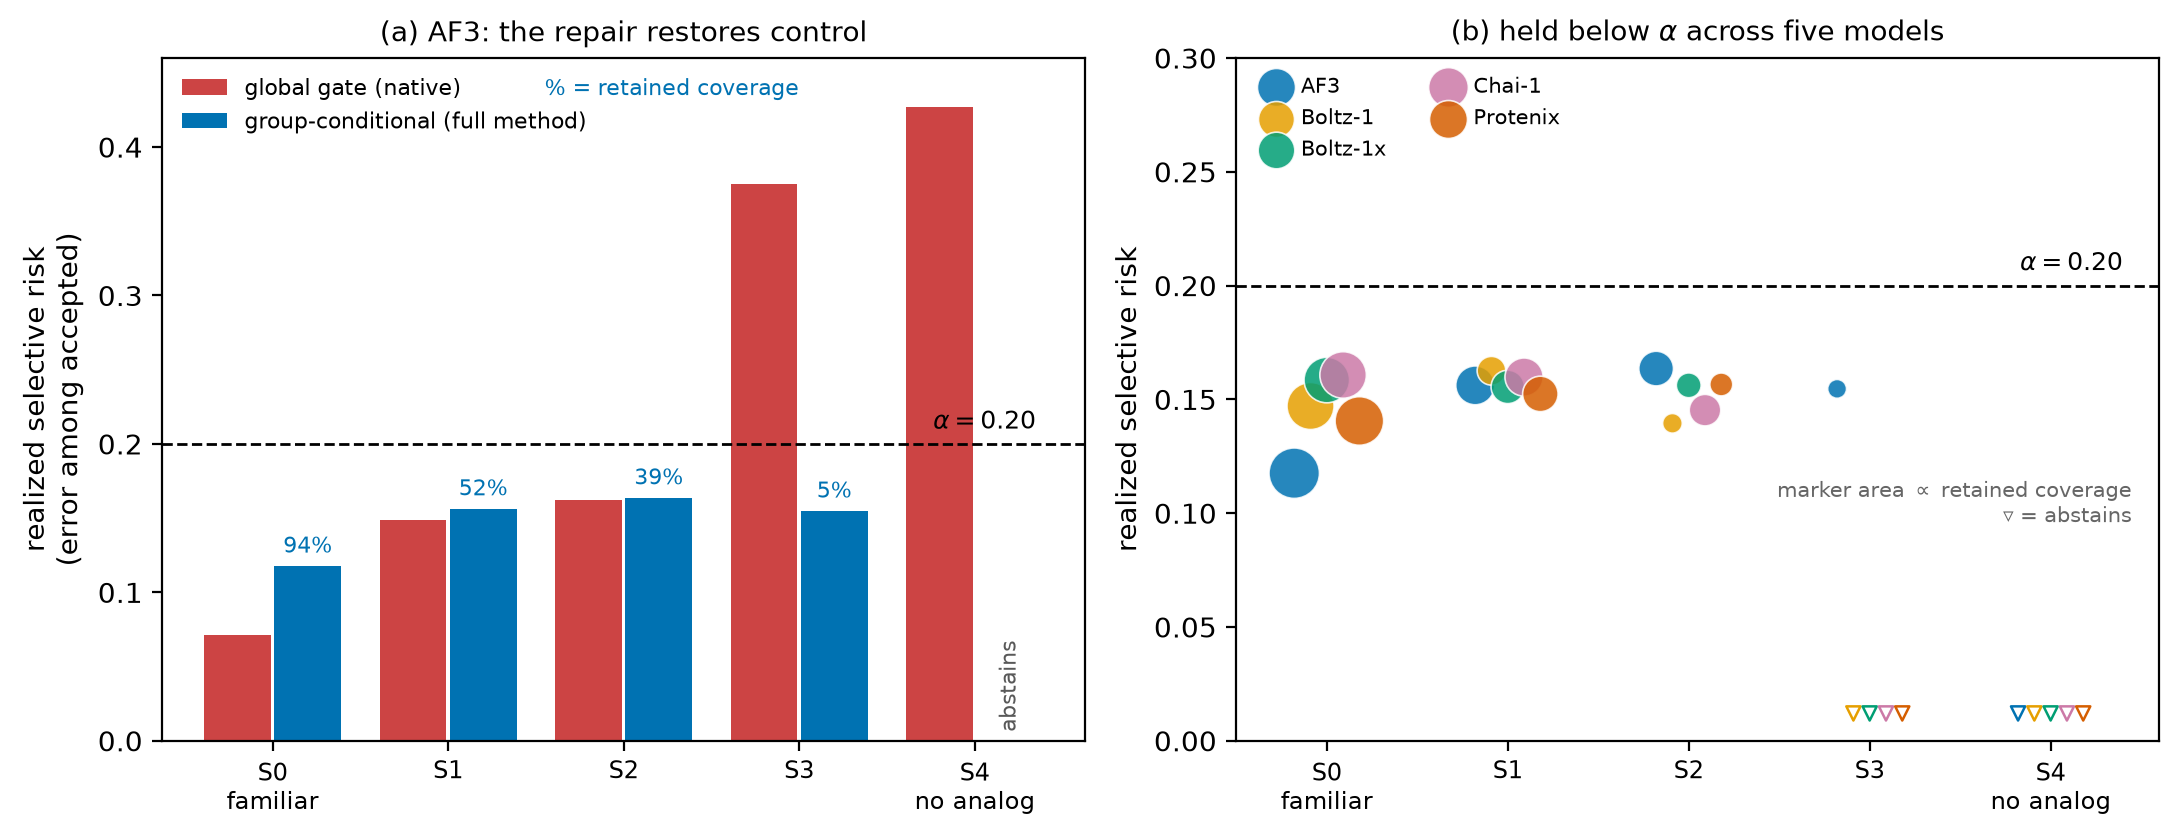
\includegraphics[width=0.98\textwidth]{../results/figures/e3_repair.png}
\caption{The repair. Group-conditional calibration holds realized selective risk at or below $\alpha=0.20$
on the strata where the marginal gate over-shoots, folding to zero coverage on the no-analog tail rather
than issuing a false certificate. Coverage labels are direct; the coverage cost grows with novelty.}
\label{fig:repair}
\end{figure}

\begin{table}[t]
\centering\small
\caption{Baselines under the novelty shift (AF3, calibrate on familiar, deploy on novel; realized risk /
coverage at $\alpha=0.20$). The field baselines break; every gate that keys calibration on novelty holds by
abstaining. Venn--Abers matches the combiner, so the shift repair does not require it.}
\label{tab:baselines}
\begin{tabular}{lcc}
\toprule
 & realized risk & coverage \\
\midrule
Fixed ipTM $\ge 0.8$ (field baseline) & $0.301$ & $0.69$ \\
Naive-transfer conformal & $0.412$ & $0.99$ \\
Accept-all & $0.417$ & $1.00$ \\
\midrule
Group-conditional (combiner) & $\mathbf{0.190}$ & $0.18$ \\
Localized / continuous novelty (RLCP)~\citep{hore2024rlcp} & $\mathbf{0.187}$ & $0.44$ \\
Per-stratum Venn--Abers~\citep{vovk2013vennabers} & $\mathbf{0.166}$ & $0.24$ \\
\bottomrule
\end{tabular}
\end{table}

\textbf{The label cost, as a design curve.} Group-conditional repair spends target labels, and how many
depends on what is being certified. For the binary pose label the count is a sufficient statistic and the
exact binomial tail is its exact inversion, so on the feasible strata it certifies at a median of $38$
independent target-labels against $60$ for a Hoeffding-Bentkus bound and $102$ for pure Hoeffding. But $38$
is a \emph{familiar}-stratum price. Figure~\ref{fig:labelcost} turns the cost into a design tool: certified
coverage as a function of the label budget $n_g$, per stratum. With the native score, no budget buys usable
coverage on the novel strata, because there the rule fails, not the estimate of it, the impossibility made
empirical. The combined score, a partly novelty-aware re-score and so on the achievability side, unlocks the
moderate strata: AF3 reaches $22\%$ certified coverage on $S_1$ at $\sim\!80$ in-stratum labels and $83\%$
with the full pool, and $77\%$ on $S_2$, while $S_3$ needs close to the full label pool for any coverage at
all. The combined score raises the ceiling, not the label floor.

\begin{figure}[t]
\centering
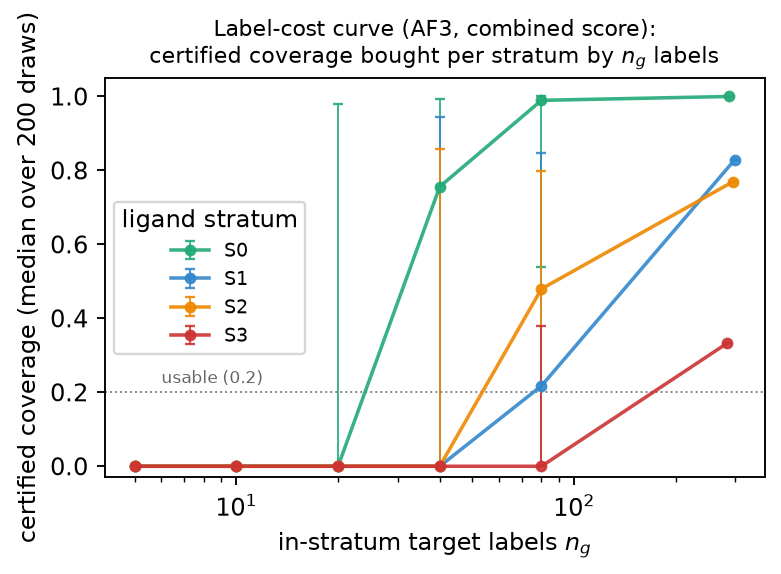
\includegraphics[width=0.62\textwidth]{../results/figures/label_cost.png}
\caption{Label-cost curve. Certified coverage bought by $n_g$ in-stratum target-labels, per ligand stratum
(AF3, combined score, median over $200$ draws with a $90\%$ band). Moderate novelty ($S_1,S_2$) is
certifiable at a measured label budget; the near-novel $S_3$ is label-starved even at the full pool.}
\label{fig:labelcost}
\end{figure}

\textbf{Deployment-computable stratifier.} The repair needs a novelty stratum at deployment, but the
oracle similarity is computed against the model's training set, which for a closed model like AF3 a user
cannot enumerate. A public proxy built from the count of pre-cutoff PDB analogs (deposition recency and
protein sequence identity are at chance) recovers the oracle stratification with rank correlation $0.59$
and $83\%$ adjacent agreement, and matches oracle per-stratum control on the low and moderate strata, but
loosens control on the near-novel tail (true-$S_3$ risk $0.23\!\to\!0.37$). The binding limit, however, is
not the proxy: even the \emph{oracle} group-conditional gate leaves the no-analog stratum above $\alpha$
(risk $0.60$). So for closed-training models the repair is deployable one stratum out with a public proxy,
and the extreme novel tail is uncertifiable by stratification alone, whether the stratifier is proxy or
oracle. That, not a missing training set, is the honest ceiling.

\textbf{A label-free worst-subpopulation certificate.} When the novel subpopulation is unnamed we control
the conditional value-at-risk of the accepted loss, the mean error of its worst $(1-\beta)$-fraction. For
the binary label $\mathrm{CVaR}_\beta=\min(1,r/(1-\beta))$ with accepted error rate $r$, so a finite-sample
bound on $r$~\citep{bates2021rcps} yields a $\mathrm{CVaR}_\beta$ bound at every $\beta$, and by CVaR--DRO
duality this certifies that every accepted subpopulation of mass at least $m^\star=1-\beta^\star$ has error
$\le\alpha$~\citep{snell2022qrc}, with no stratum labels and no importance weights, reparameterizing to a
$\chi^2$ robustness radius $\rho^\star$~\citep{cauchois2024}. A Bonferroni $\delta/K$ correction gives one
certificate jointly across the five models (at $20\%$ coverage, $m^\star\le0.52$ and $\rho^\star\ge0.10$).
This certificate is a real capability on moderate shift and, we report plainly, \emph{vacuous exactly where
it is most needed}: on deploy-to-novel $m^\star\!\to\!1$ for most models, so the label-free certificate
cannot rescue the novel tail either.

\textbf{Match the certifier to the loss.} On the \emph{graded} loss $\min(\text{RMSD},4)/4$ a
variance-adaptive betting bound~\citep{waudbysmith2024betting} certifies a usable operating point where a
distribution-free bound certifies none: AF3 certifies $43\%$ coverage at a $1$\,\AA\ mean-RMSD target with
realized capped-mean RMSD $0.90$\,\AA, against essentially zero ($0.04\%$) for a worst-case Hoeffding bound;
the empirical guarantee coverage over $120$ resamples is $0.90$. The reliability layer is therefore not tied
to the $2$\,\AA\ convention, and ``$1$\,\AA'' is an actionable operating point where ``$\alpha=0.20$'' is not.

\textbf{Certificate ledger.} Table~\ref{tab:ledger} states, per claim, the $\delta$, the multiplicity
method, the $n$, and whether the claim is joint or per-model, so no favorable $\delta$ is chosen per claim.
The $55$-cell drift grid ($5$ models $\times$ $11$ axis-strata: $4$ ligand $+$ $4$ pocket $+$ $3$ temporal
non-reference strata) uses a Romano-Wolf step-down bootstrap~\citep{romanowolf2005} at family-wise $0.10$;
all $40$ structural cells survive, an effect-dominated family, and only $2$ of $15$ temporal cells do.

\begin{table}[t]
\centering\small
\caption{Certificate ledger. $K=5$ models; joint claims split $\delta$ by a Bonferroni union bound.}
\label{tab:ledger}
\begin{tabular}{lllll}
\toprule
Claim & $\delta$ & multiplicity & $n$ (unit) & scope \\
\midrule
Global / LOTO gate & $0.10$ & fixed-sequence LTT & target-labels & per-model \\
Joint LOTO gate & $0.02$ & Bonferroni $\delta/K$ & target-labels & joint (5 models) \\
CVaR / DRO bound & $0.02$ & Bonferroni $\delta/K$ & accepted poses & joint (5 models) \\
Betting bound (graded) & $0.10$ & anytime-valid (Ville) & accepted poses & per-model \\
Drift grid & $0.10$ & Romano-Wolf step-down & $55$ cells & family-wise \\
``For every model'' effects & $0.10$ & intersection-union & per-model $p$ & no penalty \\
\bottomrule
\end{tabular}
\end{table}

\section{Utility, priced and leakage-free}\label{sec:utility}
\textbf{Ranking utility.} Every utility number is target-grouped. Under a nested leave-one-target-out
protocol (outer GroupKFold on system id; within each training fold a grouped fit/calibration split, so the
combiner, the threshold, and the test target are mutually disjoint), the combined-score gate keeps
$\mathbf{73\%}$ of AF3 poses at certified risk $\le\alpha$ (realized $0.176$, Hoeffding-Bentkus upper bound
$0.192$), where the native gate keeps $\mathbf{20\%}$; at the stringent $\alpha=0.10$ the combined gate
keeps $13\%$ at realized risk $0.066$. Chai and Protenix native gates abstain entirely under this
leakage-free protocol, the honest native limit the combined score recovers ($64\%$ and $57\%$ coverage).
These replace an earlier held-out-split pair ($71\%$ vs.\ $22\%$) that a pooled split would have leaked; the
grouped protocol shares zero targets between calibration and test, where a random row split leaks $95\%$.
The leave-one-target-out risks come with certified upper bounds and pass/fail per model
(Table~\ref{tab:loto}).

\begin{table}[t]
\centering\small
\caption{Leakage-free nested-LOTO gate, native vs.\ combined score ($\alpha=0.20$, $\delta=0.10$): coverage,
realized risk, exact Clopper-Pearson upper bound, and folds holding. Chai/Protenix native gates abstain.}
\label{tab:loto}
\begin{tabular}{lcccccc}
\toprule
 & \multicolumn{3}{c}{native} & \multicolumn{3}{c}{combined} \\
 & cov & risk & CP$_{90}^{\uparrow}$ & cov & risk & CP$_{90}^{\uparrow}$ \\
\midrule
AF3 & $0.20$ & $0.189$ & $0.218$ & $0.73$ & $0.176$ & $0.190$ \\
Boltz-1 & $0.21$ & $0.188$ & $0.219$ & $0.60$ & $0.181$ & $0.199$ \\
Boltz-1x & $0.20$ & $0.164$ & $0.194$ & $0.48$ & $0.182$ & $0.202$ \\
Chai-1 & \multicolumn{3}{c}{abstains} & $0.64$ & $0.178$ & $0.195$ \\
Protenix & \multicolumn{3}{c}{abstains} & $0.57$ & $0.182$ & $0.199$ \\
\bottomrule
\end{tabular}
\end{table}

\textbf{A decision curve retires the choice of $\alpha$.} Rather than defend a level, we sweep the cost
ratio $\lambda=\text{cost(act on a wrong pose)}/\text{cost(abstain on a right pose)}$ and plot net benefit
(Fig.~\ref{fig:decision}). The conformal gate is best for $\lambda\in[0.65,4.55]$ (AF3; every model shows
the same window), dominating a fixed-ipTM threshold at \emph{every} $\lambda$ and beating accept-all once
wrong poses are more than $\sim\!0.65\times$ as costly as a missed right one. The layer's job is the
high-cost regime, which is where a delivered pose that must be trusted lives.

\begin{figure}[t]
\centering
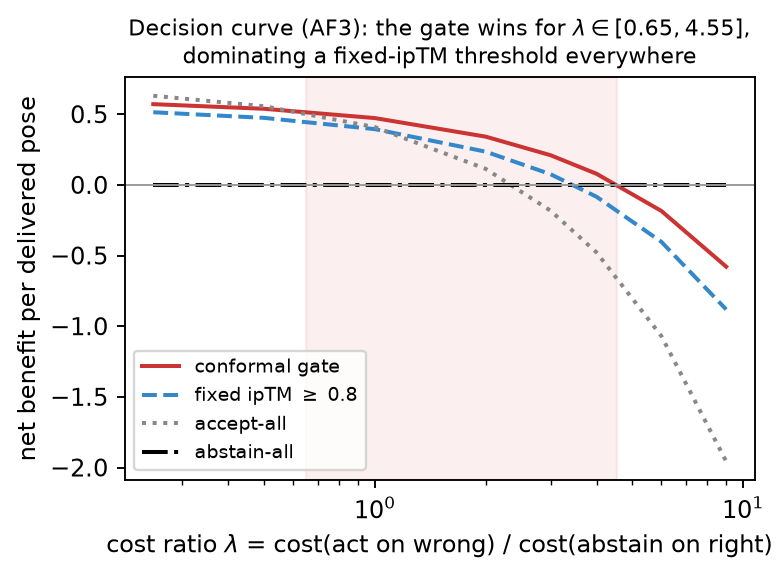
\includegraphics[width=0.62\textwidth]{../results/figures/decision_curve.png}
\caption{Decision curve (AF3). Net benefit per delivered pose vs.\ the cost ratio $\lambda$; the shaded band
is where the conformal gate is the best of the four strategies. It dominates a fixed-ipTM threshold
everywhere and serves the high-cost regime, so there is no single $\alpha$ to defend.}
\label{fig:decision}
\end{figure}

\textbf{A non-circular quality, honestly conditioned.} Accepted-pose purity is $1-$ selective risk by
construction, so it cannot show the gate buys anything past the guarantee. Interaction-fingerprint recovery,
the fraction of the crystal's protein-ligand contacts a pose reproduces, is a different quantity a
medicinal chemist reads. Pooling all accepted against all rejected poses shows a large gap ($0.19$ for
AF3), but most of that is the accepted set being enriched for low-RMSD poses. Conditioning removes the
confound: \emph{within} the sub-$2$\,\AA\ set the accepted-minus-rejected recovery gap is $+0.02$ to
$+0.04$, and a regression of recovery on RMSD with the gate as a covariate leaves a gate coefficient of
$+0.03$ to $+0.07$ (all five $90\%$ intervals excluding zero). So the gate buys a small but robust
non-circular interaction-recovery lift, once the RMSD confound is removed. Separately, the accepted set is
PoseBusters-valid at a higher rate than the rejected set for every model (AF3 $0.77$ vs.\ $0.58$), a free
strengthening; certifying the joint label (RMSD $\le2$\,\AA\ \emph{and} physically valid) directly is
expensive because the confidence ranks for correctness, not validity, and we report that cost rather than
hide it.

\section{Generality and limitations}\label{sec:general}
\textbf{Pseudo-prospective.} Freezing calibration on everything deposited before $2023$-05-31 and deploying
on everything after, with no stratum information at calibration, the native gate holds realized post-cutoff
risk $\le\alpha$ (or its Clopper-Pearson upper bound does) for four of five models and the combined gate
for three, with realized-minus-expected risk in $[-0.04,+0.00]$; the abstentions are honest
non-certifications, not violations. This is a recency transfer, complementary to the structural story, and
inherits the caveat that Runs N' Poses is entirely post-cutoff.

\textbf{Cross-dataset.} Recast as risk control rather than ranking, a threshold frozen on Runs N' Poses and
deployed on regenerated FoldBench~\citep{foldbench} Protenix predictions does not overshoot $\alpha$ on
either subset, but it certifies almost nothing on the $52$ low-homology targets (accepts $3$, coverage
$6\%$, Clopper-Pearson risk upper bound $0.63$), so the failure mode of cross-dataset transfer is coverage
starvation, not risk violation, the coverage collapse of Sec.~\ref{sec:break} reproduced on a second
dataset. The interface-ipTM gate out-ranks a \texttt{ranking\_score} control (AURC $0.380$ vs.\ $0.454$) but
their $90\%$ bootstrap intervals overlap, and the regenerated model's self-scored top-1 success ($0.40$)
differs from the released $0.57$, so this stays a directional transfer check, feature and label
self-consistent within the one run. A third dataset would need a benchmark that releases ipTM and
PoseBusters per pose; where none is available we state that concrete community ask rather than overclaim
generality.

\textbf{Limitations.} The no-analog tail is uncertifiable by every method, where abstention is the only
action. The best ranker in our screening analysis (SI), a Boltz-2 affinity head, carries no coverage
guarantee: extending the framework to certify an affinity ranker (which needs an affinity-error label) is
the top open problem. All evaluation is retrospective; a prospective screen with wet-lab confirmation is the
natural next step.

\section{Conclusion}
Co-folding confidence becomes a risk-controlled decision only when the guarantee is audited where it fails.
On structural novelty a marginally valid gate under-controls error more than twofold, and on $35$ of $47$
zero-frontier cells no threshold on the frozen score is certifiable at any coverage. An exact decomposition
explains why: the concept gap that opens there closes under in-stratum recalibration but under no
training-free reweighting. Three honest bottom lines follow. Co-folding confidence is certifiable on the
familiar strata. It is extendable one stratum outward at a measured price, a median of $38$ in-stratum
target structures, and with a public proxy stratifier for closed-training models. And on the extreme novel
tail, exactly where a program most needs a guarantee, neither stratification nor a label-free certificate
can supply one, so abstention is the certified action. The layer runs on frozen models' released
predictions on CPU and ships as certificate cards per model and novelty stratum.

\textbf{Data and code availability.} Code and calibration tables are at
\url{https://github.com/rikhinkavuru/foldgate} under an OSI-approved license; a one-command \texttt{make
repro} reproduces the tabular results from a pinned environment (\texttt{uv.lock}, fixed seeds), with the
screening, cross-model, and structure-feature arms opt-in because they consume larger released artifacts.
Runs N' Poses is at Zenodo (\texttt{10.5281/zenodo.14794785}); the regenerated FoldBench predictions and
self-scored labels are at Zenodo (\texttt{10.5281/zenodo.21417241}); the screening scores are
from~\citet{shen2026vs}. The coverage grid, fixed-sequence order, binning, and endpoints are frozen in a
timestamped pre-registration file in the repository.

\textbf{Funding.} No external funding. \textbf{Competing interests.} The author declares none.
\textbf{Broader impact.} The layer is a decision gate for drug-discovery pipelines; its central message is
conservative (abstain where the guarantee is vacuous), and its main risk is misuse as a certificate on the
novel tail, which Secs.~\ref{sec:frontier}--\ref{sec:repair} explicitly forbid.

\small
\bibliographystyle{unsrtnat}
\begin{thebibliography}{99}
\bibitem{angelopoulos2021ltt} A. Angelopoulos, S. Bates, E. Cand\`es, M. Jordan, L. Lei.
Learn then Test: Calibrating Predictive Algorithms to Achieve Risk Control. arXiv:2110.01052 (preprint), 2021.
\bibitem{bates2021rcps} S. Bates, A. Angelopoulos, L. Lei, J. Malik, M. Jordan.
Distribution-Free, Risk-Controlling Prediction Sets. J. ACM 68(6), 2021.
\bibitem{tibshirani2019} R. Tibshirani, R. Foygel Barber, E. Cand\`es, A. Ramdas.
Conformal Prediction Under Covariate Shift. NeurIPS, 2019.
\bibitem{snell2022qrc} J. Snell, T. Zollo, Z. Deng, T. Pitassi, R. Zemel.
Quantile Risk Control. arXiv:2212.13629 (preprint), 2022.
\bibitem{hore2024rlcp} R. Hore, R. Foygel Barber. Conformal Prediction with Local Weights:
Randomization Enables Robust Guarantees. J. R. Stat. Soc. B, 2024.
\bibitem{barber2021limits} R. Foygel Barber, E. Cand\`es, A. Ramdas, R. Tibshirani.
The Limits of Distribution-Free Conditional Predictive Inference. Information and Inference 10(2), 2021.
\bibitem{geifman2017} Y. Geifman, R. El-Yaniv. Selective Classification for Deep Neural Networks. NeurIPS, 2017.
\bibitem{rnp} A. Morehead, N. Giri, et al. (Runs N' Poses). A benchmark of released co-folding predictions
with training-similarity annotations. Zenodo 10.5281/zenodo.14794785, 2025.
\bibitem{foldbench} Q. Feng, S. Xu, et al. FoldBench: a low-homology benchmark for biomolecular structure
prediction. Nature Communications, 2025.
\bibitem{shen2026vs} C. Shen, et al. Unlocking the application potential of AlphaFold3-like approaches in
virtual screening. Chemical Science, 2026. Zenodo 10.5281/zenodo.17568813.
\bibitem{af3} J. Abramson, et al. Accurate structure prediction of biomolecular interactions with
AlphaFold3. Nature 630, 2024.
\bibitem{chai} Chai Discovery Team. Chai-1: Decoding the Molecular Interactions of Life. bioRxiv (preprint), 2024.
\bibitem{protenix} ByteDance AML AI4Science Team. Protenix: Advancing Structure Prediction Through a
Comprehensive AlphaFold3 Reproduction. bioRxiv (preprint), 2025.
\bibitem{codrug} K. Nguyen, et al. CoDrug: Conformal Drug Property Prediction with Density Estimation
under Covariate Shift. NeurIPS, 2023.
\bibitem{jin2023selection} Y. Jin, E. Cand\`es. Selection by Prediction with Conformal p-values. JMLR, 2023
(arXiv:2210.01408).
\bibitem{bai2026score} T. Bai, Y. Jin. Conformal Selective Prediction with General Risk Control.
arXiv:2603.24704 (preprint), 2026.
\bibitem{mondrian} V. Vovk. Conditional Validity of Inductive Conformal Predictors. Machine Learning 92, 2013
(Mondrian / group-conditional conformal).
\bibitem{vovk2013vennabers} V. Vovk, I. Petej. Venn-Abers Predictors. UAI, 2014.
\bibitem{crcgupta} V. Kotte. When Can Conformal Risk Control Certify LLM Outputs? Bounds, Impossibility, and
Adaptation for Structured Generation. arXiv:2606.29054 (preprint), 2026 (concurrent, independent
reweighting-invariant selective-risk floor, LLM domain).
\bibitem{boltz} J. Wohlwend, et al. Boltz-1: Democratizing Biomolecular Interaction Modeling. bioRxiv
(preprint), 2024. Boltz-1x (confidence-refined) and Boltz-2 (affinity), 2025; versions used are recorded in
the repository.
\bibitem{vovk2005} V. Vovk, A. Gammerman, G. Shafer. Algorithmic Learning in a Random World. Springer, 2005.
\bibitem{cauchois2024} M. Cauchois, S. Gupta, A. Ali, J. Duchi. Robust Validation: Confident Predictions
Even When Distributions Shift. JASA, 2024.
\bibitem{bendavid2010} S. Ben-David, J. Blitzer, K. Crammer, A. Kulesza, F. Pereira, J. Vaughan.
A Theory of Learning from Different Domains. Machine Learning 79, 2010.
\bibitem{angelopoulos2024crc} A. Angelopoulos, S. Bates, A. Fisch, L. Lei, T. Schuster.
Conformal Risk Control. ICLR, 2024.
\bibitem{incoherence} T. Valentin, A. Madadi, G. Sapia, M. B\"ohme. Incoherence as Oracle-less Measure of
Error in LLM-Based Code Generation. AAAI, 2026 (arXiv:2507.00057, preprint).
\bibitem{credal} V. Venkatesh, E. H\"ullermeier, B. Bischl, M. Rezaei. Structured Credal Learning.
arXiv:2603.14070 (preprint), 2026.
\bibitem{consensusdocking} R. Houston, M. Walkinshaw. Consensus Docking: Improving the Reliability of
Docking in a Virtual Screening Context. J. Chem. Inf. Model. 53(2), 2013.
\bibitem{waudbysmith2024betting} I. Waudby-Smith, A. Ramdas. Estimating Means of Bounded Random Variables by
Betting. J. R. Stat. Soc. B, 2024 (arXiv:2010.09686).
\bibitem{romanowolf2005} J. Romano, M. Wolf. Stepwise Multiple Testing as Formalized Data Snooping.
Econometrica 73, 2005.
\end{thebibliography}

\appendix
\section{Proof of the decomposition, and the ties bracket}\label{app:proof}
\small
\textbf{Setup.} Frozen score $s=s(X)$, error label $Y\in\{0,1\}$, accept region $A_\tau=\{s\ge\tau\}\in
\sigma(X)$. A training-free reweighting has weights $w=w(X)\ge0$ that are $\sigma(X)$-measurable and use no
target labels. Assume $s$ has no atom at the operating threshold, so for each coverage $c$ there is a unique
$\tau_c$ with $Q(s\ge\tau_c)=c$; real scores carry ties handled by boundary randomization, under which the
equalities become $\le/\ge$ brackets, and Sec.~\ref{sec:decomp} bounds the bracket empirically ($0$ on the
ranking-score gate, $\le0.7\%$ coverage on ipTM).

\textbf{Lemma (reweighting sees only the source labels).} For any such $w$, the reweighted plug-in selective
risk is $\widetilde{E}^w(\tau)=\mathbb{E}_P[w\,Y\,\mathbf{1}_{A_\tau}]/\mathbb{E}_P[w\,\mathbf{1}_{A_\tau}]=
\mathbb{E}_{Q_w}[\eta_P\mid A_\tau]$, with $dQ_w\propto w\,dP_X$. \emph{Proof.} $w$ and
$\mathbf{1}_{A_\tau}$ are $\sigma(X)$-measurable, so tower over $X$:
$\mathbb{E}_P[w\,Y\,\mathbf{1}_{A_\tau}]=\mathbb{E}_P[w\,\eta_P\,\mathbf{1}_{A_\tau}]$; normalize. The target
conditional $\eta_Q$ cannot appear. $\square$

\textbf{Proposition.} At coverage $c$: (a) $R_Q(\tau_c)=R_{\mathrm{ref}}(\tau_c)+\bar\Delta_c$ with
$R_{\mathrm{ref}}(\tau_c)=\mathbb{E}_Q[\eta_P\mid A_{\tau_c}]$ and $\bar\Delta_c=\mathbb{E}_Q[\eta_Q-\eta_P
\mid A_{\tau_c}]$; (b) any $w$ realizing coverage $c$ accepts exactly $A_{\tau_c}$, so its realized risk
equals $R_Q(\tau_c)$, independent of $w$; (c) with oracle weights the certificate of the Lemma equals
$R_{\mathrm{ref}}(\tau_c)$, under-reporting the realized risk by exactly $\bar\Delta_c$; (d) level $\alpha$
is achievable at coverage $c$ by some training-free reweighting iff $\bar\Delta_c\le\alpha-
R_{\mathrm{ref}}(\tau_c)$. \emph{Proof.} (a) $A_{\tau_c}\in\sigma(X)$, so $R_Q(\tau_c)=\mathbb{E}_Q[\eta_Q
\mid A_{\tau_c}]$; add and subtract $\mathbb{E}_Q[\eta_P\mid A_{\tau_c}]$. (b) The no-atom assumption pins
$\tau_c$ from $c$; realized risk is a functional of $(Q,\tau_c)$ alone. (c) Lemma with $w^\star=dQ_X/dP_X$
gives $Q_{w^\star}=Q$. (d) is (a)+(b). $\square$ The statement is coverage-pinned and binds only scalar
thresholds of a fixed score with covariate-measurable weights; re-scoring on $\nu$ or a per-stratum
threshold escapes it (the achievability side), and in-stratum split calibration~\citep{vovk2005} gives
stratum-conditional miscoverage $\le 1/(n_g{+}1)$ regardless of drift, with the ratio functional controlled
by Learn-then-Test at the finite-sample cost the label-cost curve measures.

\section{Benchmark and validation details}\label{app:bench}
\small The synthetic generator draws a stratum from a tilted $\nu$-marginal, a score logit
$z\sim\mathcal{N}(m_0-E\nu,\sigma^2)$, and a label with
$P(Y{=}1)=\epsilon+(1-2\epsilon)\,\mathrm{sigmoid}(\beta_0+\beta_1 z-D_{\mathrm{eff}}\nu)$, isolating
covariate shift ($E$), concept drift ($D$), and an error floor ($\epsilon$); every proposition quantity is
available in closed form and cross-checked by Monte Carlo. The real benchmarks reduce any classifier to
$(s,y,\nu)$; realized worst-stratum selective risk at $\alpha=0.20$: elec2 marginal $0.31$,
weighted-conformal $0.34$, group-conditional $0.20$; ACS~Income marginal $0.23$, weighted-conformal $0.20$,
group-conditional $0.20$, the reliability drift separating the two being $0.36$ (elec2, concept) against
$0.05$ (ACS, covariate).

\section{A benchmark-integrity note for cross-model pose geometry}\label{app:integrity}
\small Recomputing pose RMSD in a common frame carries a silent trap. Runs N' Poses ships only the system's
receptor chain while co-folding models predict the full biological assembly, so a chain-ordinal
superposition can land the ligand in the wrong protomer of a homodimer: the backbone still fits
(superposition residual $\sim\!0.3$\,\AA) while the ligand sits tens of \AA ngstr\"om away. Neither the
residual nor a triangle-inequality consistency check detects it, and a distance-consistency check passed at
$0/13{,}146$ while $21\%$ of recomputed distances and $15\%$ of binary correctness labels were wrong. Only
comparison against the shipped BiSyRMSD label exposes it; restricting to single-chain receptors with an
unambiguous ligand copy raises agreement from Spearman $0.620$ to $0.995$ and defines the $6{,}163$-instance
subset any recomputed-geometry result in this paper uses (Table~\ref{tab:provenance}). We flag this for
reuse; a symmetry-aware chain assignment is the general fix.

\end{document}
